\begin{abstract}
Despite the recent improvements in admissible heuristic search techniques
in classical planning, it is known that the the exponential growth of
search plateau in A* is unavoidable even under the optimistic assumption.
 % 
We investigate various existing myth on tiebreaking
 strategies and propose simple yet effective methods for improving the
 search performance within plateau.
 % 
 % 
 They do not depend on any particular heuristic, nor
 on multi-heuristic portfolio.
 They work even if the heuristic
 function no longer provides useful information.
 % Moreover, they do not even try to obtain any further information from
 % the domain.
 We empirically evaluate our strategies against state-of-the-art admissible planner.
\end{abstract}

Since the advent of delete-relaxation and abstraction heuristics in
admissible Classical Planning, much of the interest was focused on improving
the accuracy of these heuristic functions to prune more nodes from the
search space.
% 
However, recent work by Helmert and Roger
\shortcite{helmert2008good} claims that, even with an optimistic
assumption of \emph{almost-perfect heuristics}, \astar still has an
exponentially large plateau. They conclude that the further performance
improvement requires the techniques orthogonal to the heuristic
function, such as symmetry breaking, domain reduction, factored planning
etc.

The contribution of this paper is a new class of
tiebreaking strategy for \astar.
It is a heuristic-agnostic improvement and thus 
falls into above category of techniques.
It trivially maintains admissibility because it works only within the
same f-value and does not alter the expansion order wrto f-value.
% such technique.
% tiebreaking strategy for \astar.
% Our tiebreaking strategies fall into this category.

% The attention to the search algorithm itself is relatively small since
% most literature depends on bare \astar.  This was because variations of
% best first search focus on different requirements, such as IDA* on
% linear space, WA*/Lazy-A*/GBFS/EHC on trading speed for optimality, RWA*
% on replanning, etc., and not on improving upon \astar itself.

% maintaining all of its charactristics: memory-greedy yet efficient
% optimal algorithm.

More specifically, we show several important findings regarding the
existing tiebreaking strategy for \astar as follows.
% 
First, in implementing the open list of \astar, priority queue based on
LIFO-buckets is more efficient than that of FIFO-buckets.
% 
Second, with LIFO-based implementation, $h$-based tiebreaking which
frequently appears in the heuristic search literatures have little
impact on the performance.
% 
Third, the LIFO-based bucket implementation and $h$-based tiebreaking
both share the greedy search pattern within the plateau of the
search space, and thus one crucial essense of tiebreaking is the
\emph{depth within the plateau}.

The rest of paper is organized as follows: The next section describes the
preliminary background of \astar.
Next we compares several trivially-simple and well-known tiebreaking
methods on top of Fast Downward to show that even such a small
difference significantly affects the performance on domains with
large plateaus.
Next we propose a novel depth-aware tiebreaking methods and empirically
show that it outperforms previous strategies.
We finally conclude with a discussion on the future work.

\section{Backgrounds and Preliminary}
\label{sec-1}

\subsubparagraph{\astar and perfect heuristics}

\astar is a state of the art algorithm for finding an optimal path in the
search space represented as a graph. 
\astar returns an optimal solution when the heuristic function $h$ is
admissible, i.e., when it never overestimate the true distance to the goal
$h^*$.
% , and the nodes are first ordered according to $f$
% 
Thus, the best possible admissible heuristic function is $h^*$ itself, which is
called \emph{perfect heuristics}. However, computing $h^*$ is PSPACE-Complete,
which is as difficult as solving the problem itself and is not
practical.

%It is known that with a perfect heuristics the planner do not have to
% conduct any search: There are no multiple possibilities that the
% planner should examine on each node.

\emph{Almost perfect} heuristic function $h_c$ is a class of similar
impractical, theoretical functions which is also PSPACE-Complete to
compute \cite{helmert2008good}.  It has a constant error $c$ from the
perfect heuristic $h^*$, i.e., $h_c=h^*-c$.  The important finding by
\citeauthor{helmert2008good} is that even with this intractable and
impractical heuristic function, the number of the nodes in the last
plateau of the search becomes exponentially large as the problem size
increases.  Using this fact, they showed that relying only on the
improvement of the heuristic functions is not fruitful in the near
future, and the researchers should seek the other,
orthorgonal improvement.

These intractable heuristics are of course very hard and expensive to
compute. However, even the practical, tractable heuristic functions for
STRIPS Planning, such as \lmcut and IP-based heuristics, are so heavily
CPU intensive that they outweighs the space-greedy nature of
\astar. Also, compared to the other functions, these functions dominate
the search time over the other factors of planning algorithms, such as
node insertion and deletion.

% M\&S ?

\subsection{Tie Breaking Criteria in \astar}

% Compared to the other algorithms which
% guarantee optimality such as $IDA^*$ \cite{korf1985depth}, \astar requires a large amount of % memory to store the search nodes.

\astar stores the search nodes into two priority queues called an
\emph{open list} and a \emph{closed list}. In these queues, the search
nodes are sorted based on $f$ value, which is a sum of the actual cost
$g$ from the initial state and the cost estimate $h$ to the goal
state.
% On each iteration, \astar expands the open nodes with the
% smallest $f$ value and mark them as closed. Its successor nodes are
% accordingly inserted back to the open list or closed list, while
% sometimes the parent node is updated so that it has the shortest path
% from the initial state.

While the implementation of the priority queue varies, it has a degree
of freedom called tie-breaking, i.e. how to select the next node to open
within the same $f$.
In the current implementation of the \sota admissible planner Fast Downward (FD) \cite{Helmert2006}, the standard \astar search breaks ties based on $h$, meaning that if two nodes have the same $f$ value, the nodes with smaller $h$ will be selected, favoring the nodes with larger $g$ values (since $f=g+h$). The intension behind this is that the $h$ values are just an \emph{estimate} to the goal, while $g$ values are the \emph{actual} distance from the initial state and more reliable.

This tiebreaking strategy is very historically established and cited and
used in a lot of papers X, Y, Z. XXXXXXXYYYYY YYYYYYYYYYYYY
YYYYYYYYYYYYY YYYYYYY YYYYYY YYYYYYYY YYYYYYYYYYYY YYYYYYYYY
YYYYYYYYYYYYY YYYYYYYYYY YYYYYYYYYYYYYYYYY yYYYYYYYY YYYYYYYYYY
YYYYYYYYYYYYY yYYYYYYY YYYYYYYYYYYYYYY YYYYYYYYY

Another thing we note is that the nodes are stored in a FIFO order
within the same $h$ value. The planner selects the nodes that is inserted earlier. 
However, in fact, these tiebreaking methods are not necessary when we are only concerned with  maintaining the optimality. They are just the result of heuristic, ad-hoc selection by humans and have no theoretical background.
% In particular, we first observed that this FIFO order has not legitimate reason to support.

We therefore ran a preliminary experiments on 28 benchmark domains with
1294 problems in total, comparing simple FIFO, LIFO and Random-Order
second-level tiebreaking methods using 30 minutes runtime cutoff with
2GB memory limit.  All experiments below are conducted on Xeon
E5410@2.33GHz CPUs. We observed that even such a slightest difference
can change the performance significantly on some domains, shown in
\reftbl{f-h-coverage}. Due to the space limitation, we show only the
domains where the difference was observed. Full table is available in
the supplemental material.

\refig{f-h-eval} compares the number of
node evaluation (computations of \lmcut) by LIFO, FIFO and Random second
tiebreaking.  According to the figure, LIFO has smaller number of
evaluations than the others in Openstacks, but Random dominates the
others in Cybersec, indicating that there are no dominance relationship
between these three.  \reftbl{f-h-coverage} shows the coverage result
(number of problems solved) by each strategy.

Moreover, we also ran the same experiment but this time without $h$-based
first-level tiebreaking. Results in \reftbl{f-coverage} shows that the
coverage by LIFO-tiebreaking is almost comparable to those with $h$-based
tiebreaking.

% Note that, although LIFO dominated the others, we consider this is just by a coincidence due to our selection of problems, time limit and domains. we \emph{are not trying to claim that any of LIFO or FIFO or Random order dominates the other}. However, there are noticeable performance difference cause by these different tiebreaking strategies.

% \begin{figure}[htbp]
%  \centering \relsize{-2}
%  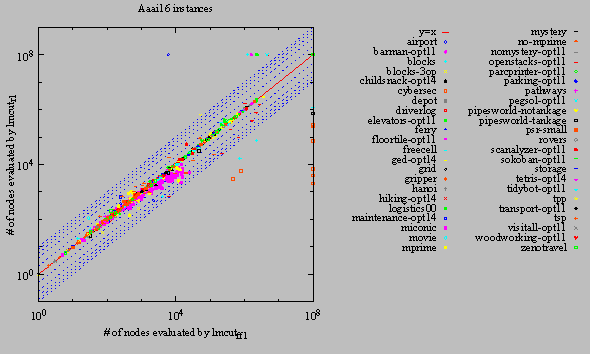
\includegraphics{tables/aaai16-evaluated-lmcut_ff-lmcut_r.pdf}
%  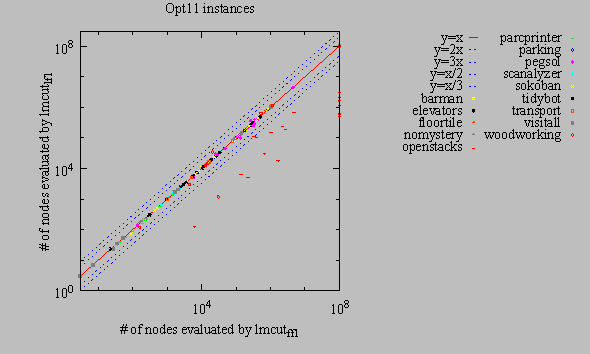
\includegraphics{tables/opt11-evaluated-lmcut_ff-lmcut_lf.pdf}
%  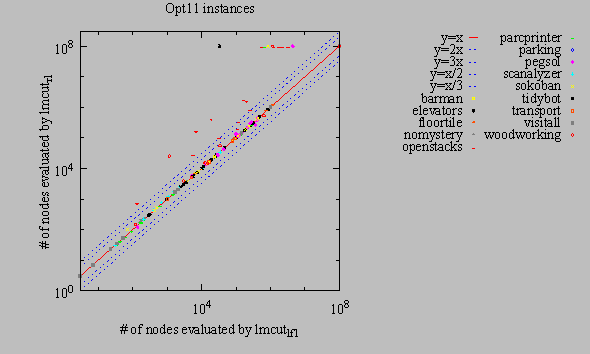
\includegraphics{tables/opt11-evaluated-lmcut_lf-lmcut_r.pdf}
%  \caption{Comparison of the number of node evaluations (computations of
%  \lmcut) by FIFO, LIFO and Random tiebreaking, on IPC2011 optimal track
%  instance. LIFO order dominates FIFO and Random order especially in
%  openstacks instances, and the gap is more than one the order of 10.}
%  \label{single-eval}
% \end{figure}
% 
\begin{table*}[htbp]
 \centering \relsize{-3}
 \begin{tabular}{|c|c|c|c|c|c|c|c|c|c|c|c|c|c||c|c|c|c|c|c|c|c|c|c|c|c||c|c||c|c|c|c|c|c|c|c|c|c|c|c||c|c|c|}
   \hline                                                                                                                           
   &  Domain & \rotatebox[origin=l]{90}{${\mbox{lmcut}}_{\mbox{ff}}$}   & \rotatebox[origin=l]{90}{${\mbox{lmcut}}_{\mbox{r}}$}   & \rotatebox[origin=l]{90}{${\mbox{lmcut}}_{\mbox{lf}}$}   & \rotatebox[origin=l]{90}{${\mbox{lmcut}}_{\mbox{${\mbox{fd}}_{\mbox{fifo}}$}}$}   & \rotatebox[origin=l]{90}{${\mbox{lmcut}}_{\mbox{${\mbox{rd}}_{\mbox{fifo}}$}}$}   & \rotatebox[origin=l]{90}{${\mbox{lmcut}}_{\mbox{${\mbox{ld}}_{\mbox{fifo}}$}}$}   & \rotatebox[origin=l]{90}{${\mbox{lmcut}}_{\mbox{${\mbox{fd}}_{\mbox{random}}$}}$}   & \rotatebox[origin=l]{90}{${\mbox{lmcut}}_{\mbox{${\mbox{rd}}_{\mbox{random}}$}}$}   & \rotatebox[origin=l]{90}{${\mbox{lmcut}}_{\mbox{${\mbox{ld}}_{\mbox{random}}$}}$}   & \rotatebox[origin=l]{90}{${\mbox{lmcut}}_{\mbox{${\mbox{fd}}_{\mbox{lifo}}$}}$}   & \rotatebox[origin=l]{90}{${\mbox{lmcut}}_{\mbox{${\mbox{rd}}_{\mbox{lifo}}$}}$}   & \rotatebox[origin=l]{90}{${\mbox{lmcut}}_{\mbox{${\mbox{ld}}_{\mbox{lifo}}$}}$}   & \rotatebox[origin=l]{90}{${\mbox{mands}}_{\mbox{ff}}$}   & \rotatebox[origin=l]{90}{${\mbox{mands}}_{\mbox{r}}$}   & \rotatebox[origin=l]{90}{${\mbox{mands}}_{\mbox{lf}}$}   & \rotatebox[origin=l]{90}{${\mbox{mands}}_{\mbox{${\mbox{fd}}_{\mbox{fifo}}$}}$}   & \rotatebox[origin=l]{90}{${\mbox{mands}}_{\mbox{${\mbox{rd}}_{\mbox{fifo}}$}}$}   & \rotatebox[origin=l]{90}{${\mbox{mands}}_{\mbox{${\mbox{ld}}_{\mbox{fifo}}$}}$}   & \rotatebox[origin=l]{90}{${\mbox{mands}}_{\mbox{${\mbox{fd}}_{\mbox{random}}$}}$}   & \rotatebox[origin=l]{90}{${\mbox{mands}}_{\mbox{${\mbox{rd}}_{\mbox{random}}$}}$}   & \rotatebox[origin=l]{90}{${\mbox{mands}}_{\mbox{${\mbox{ld}}_{\mbox{random}}$}}$}   & \rotatebox[origin=l]{90}{${\mbox{mands}}_{\mbox{${\mbox{fd}}_{\mbox{lifo}}$}}$}   & \rotatebox[origin=l]{90}{${\mbox{mands}}_{\mbox{${\mbox{rd}}_{\mbox{lifo}}$}}$}   & \rotatebox[origin=l]{90}{${\mbox{mands}}_{\mbox{${\mbox{ld}}_{\mbox{lifo}}$}}$}   & \rotatebox[origin=l]{90}{${\mbox{blind}}_{\mbox{ff}}$}   & \rotatebox[origin=l]{90}{${\mbox{blind}}_{\mbox{lf}}$}   & \rotatebox[origin=l]{90}{${\mbox{lmcut}}_{\mbox{${\mbox{ff}}_{\mbox{noh}}$}}$}   & \rotatebox[origin=l]{90}{${\mbox{lmcut}}_{\mbox{${\mbox{r}}_{\mbox{noh}}$}}$}   & \rotatebox[origin=l]{90}{${\mbox{lmcut}}_{\mbox{${\mbox{lf}}_{\mbox{noh}}$}}$}   & \rotatebox[origin=l]{90}{${\mbox{lmcut}}_{\mbox{${\mbox{fd}}_{\mbox{${\mbox{fifo}}_{\mbox{noh}}$}}$}}$}   & \rotatebox[origin=l]{90}{${\mbox{lmcut}}_{\mbox{${\mbox{rd}}_{\mbox{${\mbox{fifo}}_{\mbox{noh}}$}}$}}$}   & \rotatebox[origin=l]{90}{${\mbox{lmcut}}_{\mbox{${\mbox{ld}}_{\mbox{${\mbox{fifo}}_{\mbox{noh}}$}}$}}$}   & \rotatebox[origin=l]{90}{${\mbox{lmcut}}_{\mbox{${\mbox{fd}}_{\mbox{${\mbox{random}}_{\mbox{noh}}$}}$}}$}   & \rotatebox[origin=l]{90}{${\mbox{lmcut}}_{\mbox{${\mbox{rd}}_{\mbox{${\mbox{random}}_{\mbox{noh}}$}}$}}$}   & \rotatebox[origin=l]{90}{${\mbox{lmcut}}_{\mbox{${\mbox{ld}}_{\mbox{${\mbox{random}}_{\mbox{noh}}$}}$}}$}   & \rotatebox[origin=l]{90}{${\mbox{lmcut}}_{\mbox{${\mbox{fd}}_{\mbox{${\mbox{lifo}}_{\mbox{noh}}$}}$}}$}   & \rotatebox[origin=l]{90}{${\mbox{lmcut}}_{\mbox{${\mbox{rd}}_{\mbox{${\mbox{lifo}}_{\mbox{noh}}$}}$}}$}   & \rotatebox[origin=l]{90}{${\mbox{lmcut}}_{\mbox{${\mbox{ld}}_{\mbox{${\mbox{lifo}}_{\mbox{noh}}$}}$}}$}   & \rotatebox[origin=l]{90}{${\mbox{mands}}_{\mbox{${\mbox{ff}}_{\mbox{noh}}$}}$}   & \rotatebox[origin=l]{90}{${\mbox{mands}}_{\mbox{${\mbox{r}}_{\mbox{noh}}$}}$}   & \rotatebox[origin=l]{90}{${\mbox{mands}}_{\mbox{${\mbox{lf}}_{\mbox{noh}}$}}$}    \\
   \hline                                                                                                                           
   &  Sum &  560 &  556 &  \textbf{565} &  0 &  0 &  0 &  0 &  0 &  0 &  0 &  0 &  0 &  489 &  470 &  \textbf{496} &  0 &  0 &  0 &  0 &  0 &  0 &  0 &  0 &  0 &  402 &  \textbf{408} &  445 &  445 &  \textbf{559} &  0 &  0 &  0 &  0 &  0 &  0 &  0 &  0 &  0 &  460 &  422 &  \textbf{491}  \\
   \hline                                                                                                                           
\multirow{35}{*}{\rotatebox[origin=c]{90}{\textbf{LMcut Benchmark Suite+}}}   &  {\relsize{-1}airport(50)} &  \textbf{27} &  25 &  26 &  0 &  0 &  0 &  0 &  0 &  0 &  0 &  0 &  0 &  \textbf{9} &  \textbf{9} &  \textbf{9} &  0 &  0 &  0 &  0 &  0 &  0 &  0 &  0 &  0 &  18 &  18 &  18 &  18 &  \textbf{26} &  0 &  0 &  0 &  0 &  0 &  0 &  0 &  0 &  0 &  9 &  9 &  9  \\
   &  {\relsize{-1}barman-opt11(20)} &  0 &  0 &  0 &  0 &  0 &  0 &  0 &  0 &  0 &  0 &  0 &  0 &  \textbf{4} &  \textbf{4} &  \textbf{4} &  0 &  0 &  0 &  0 &  0 &  0 &  0 &  0 &  0 &  4 &  4 &  0 &  0 &  0 &  0 &  0 &  0 &  0 &  0 &  0 &  0 &  0 &  0 &  4 &  4 &  4  \\
   &  {\relsize{-1}blocks(35)} &  \textbf{28} &  \textbf{28} &  \textbf{28} &  0 &  0 &  0 &  0 &  0 &  0 &  0 &  0 &  0 &  \textbf{22} &  \textbf{22} &  \textbf{22} &  0 &  0 &  0 &  0 &  0 &  0 &  0 &  0 &  0 &  18 &  18 &  26 &  26 &  \textbf{27} &  0 &  0 &  0 &  0 &  0 &  0 &  0 &  0 &  0 &  21 &  19 &  \textbf{22}  \\
   &  {\relsize{-1}cybersec(19)} &  1 &  \textbf{2} &  \textbf{2} &  0 &  0 &  0 &  0 &  0 &  0 &  0 &  0 &  0 &  0 &  0 &  0 &  0 &  0 &  0 &  0 &  0 &  0 &  0 &  0 &  0 &  0 &  0 &  0 &  0 &  \textbf{1} &  0 &  0 &  0 &  0 &  0 &  0 &  0 &  0 &  0 &  0 &  0 &  0  \\
   &  {\relsize{-1}depot(22)} &  \textbf{6} &  \textbf{6} &  \textbf{6} &  0 &  0 &  0 &  0 &  0 &  0 &  0 &  0 &  0 &  \textbf{6} &  5 &  \textbf{6} &  0 &  0 &  0 &  0 &  0 &  0 &  0 &  0 &  0 &  4 &  4 &  5 &  5 &  \textbf{6} &  0 &  0 &  0 &  0 &  0 &  0 &  0 &  0 &  0 &  5 &  4 &  \textbf{6}  \\
   &  {\relsize{-1}driverlog(20)} &  \textbf{13} &  \textbf{13} &  \textbf{13} &  0 &  0 &  0 &  0 &  0 &  0 &  0 &  0 &  0 &  \textbf{12} &  \textbf{12} &  \textbf{12} &  0 &  0 &  0 &  0 &  0 &  0 &  0 &  0 &  0 &  7 &  7 &  12 &  12 &  \textbf{13} &  0 &  0 &  0 &  0 &  0 &  0 &  0 &  0 &  0 &  \textbf{12} &  11 &  \textbf{12}  \\
   &  {\relsize{-1}elevators-opt11(20)} &  \textbf{15} &  \textbf{15} &  \textbf{15} &  0 &  0 &  0 &  0 &  0 &  0 &  0 &  0 &  0 &  \textbf{13} &  12 &  \textbf{13} &  0 &  0 &  0 &  0 &  0 &  0 &  0 &  0 &  0 &  9 &  9 &  14 &  14 &  \textbf{15} &  0 &  0 &  0 &  0 &  0 &  0 &  0 &  0 &  0 &  \textbf{13} &  10 &  \textbf{13}  \\
   &  {\relsize{-1}floortile-opt11(20)} &  \textbf{6} &  \textbf{6} &  \textbf{6} &  0 &  0 &  0 &  0 &  0 &  0 &  0 &  0 &  0 &  \textbf{6} &  \textbf{6} &  \textbf{6} &  0 &  0 &  0 &  0 &  0 &  0 &  0 &  0 &  0 &  2 &  2 &  \textbf{6} &  \textbf{6} &  \textbf{6} &  0 &  0 &  0 &  0 &  0 &  0 &  0 &  0 &  0 &  5 &  4 &  \textbf{6}  \\
   &  {\relsize{-1}freecell(80)} &  \textbf{9} &  \textbf{9} &  \textbf{9} &  0 &  0 &  0 &  0 &  0 &  0 &  0 &  0 &  0 &  \textbf{17} &  15 &  \textbf{17} &  0 &  0 &  0 &  0 &  0 &  0 &  0 &  0 &  0 &  15 &  15 &  8 &  \textbf{9} &  \textbf{9} &  0 &  0 &  0 &  0 &  0 &  0 &  0 &  0 &  0 &  15 &  14 &  \textbf{16}  \\
   &  {\relsize{-1}grid(5)} &  \textbf{1} &  \textbf{1} &  \textbf{1} &  0 &  0 &  0 &  0 &  0 &  0 &  0 &  0 &  0 &  \textbf{2} &  \textbf{2} &  \textbf{2} &  0 &  0 &  0 &  0 &  0 &  0 &  0 &  0 &  0 &  1 &  1 &  \textbf{1} &  \textbf{1} &  \textbf{1} &  0 &  0 &  0 &  0 &  0 &  0 &  0 &  0 &  0 &  2 &  2 &  2  \\
   &  {\relsize{-1}gripper(20)} &  \textbf{6} &  \textbf{6} &  \textbf{6} &  0 &  0 &  0 &  0 &  0 &  0 &  0 &  0 &  0 &  \textbf{20} &  \textbf{20} &  \textbf{20} &  0 &  0 &  0 &  0 &  0 &  0 &  0 &  0 &  0 &  7 &  7 &  \textbf{6} &  \textbf{6} &  \textbf{6} &  0 &  0 &  0 &  0 &  0 &  0 &  0 &  0 &  0 &  8 &  6 &  \textbf{20}  \\
   &  {\relsize{-1}hanoi(30)} &  \textbf{12} &  \textbf{12} &  \textbf{12} &  0 &  0 &  0 &  0 &  0 &  0 &  0 &  0 &  0 &  \textbf{14} &  \textbf{14} &  \textbf{14} &  0 &  0 &  0 &  0 &  0 &  0 &  0 &  0 &  0 &  12 &  12 &  \textbf{12} &  \textbf{12} &  \textbf{12} &  0 &  0 &  0 &  0 &  0 &  0 &  0 &  0 &  0 &  14 &  14 &  14  \\
   &  {\relsize{-1}logistics00(28)} &  \textbf{20} &  \textbf{20} &  \textbf{20} &  0 &  0 &  0 &  0 &  0 &  0 &  0 &  0 &  0 &  \textbf{20} &  \textbf{20} &  \textbf{20} &  0 &  0 &  0 &  0 &  0 &  0 &  0 &  0 &  0 &  10 &  10 &  16 &  16 &  \textbf{19} &  0 &  0 &  0 &  0 &  0 &  0 &  0 &  0 &  0 &  \textbf{20} &  17 &  \textbf{20}  \\
   &  {\relsize{-1}miconic(150)} &  \textbf{140} &  \textbf{140} &  \textbf{140} &  0 &  0 &  0 &  0 &  0 &  0 &  0 &  0 &  0 &  \textbf{73} &  72 &  \textbf{73} &  0 &  0 &  0 &  0 &  0 &  0 &  0 &  0 &  0 &  49 &  \textbf{50} &  68 &  68 &  \textbf{140} &  0 &  0 &  0 &  0 &  0 &  0 &  0 &  0 &  0 &  68 &  68 &  \textbf{73}  \\
   &  {\relsize{-1}mprime(35)} &  \textbf{21} &  \textbf{21} &  \textbf{21} &  0 &  0 &  0 &  0 &  0 &  0 &  0 &  0 &  0 &  23 &  23 &  \textbf{24} &  0 &  0 &  0 &  0 &  0 &  0 &  0 &  0 &  0 &  19 &  19 &  20 &  19 &  \textbf{22} &  0 &  0 &  0 &  0 &  0 &  0 &  0 &  0 &  0 &  \textbf{23} &  22 &  \textbf{23}  \\
   &  {\relsize{-1}mystery(30)} &  \textbf{16} &  15 &  \textbf{16} &  0 &  0 &  0 &  0 &  0 &  0 &  0 &  0 &  0 &  15 &  15 &  \textbf{16} &  0 &  0 &  0 &  0 &  0 &  0 &  0 &  0 &  0 &  15 &  15 &  15 &  15 &  \textbf{16} &  0 &  0 &  0 &  0 &  0 &  0 &  0 &  0 &  0 &  15 &  15 &  15  \\
   &  {\relsize{-1}nomystery-opt11(20)} &  \textbf{14} &  \textbf{14} &  \textbf{14} &  0 &  0 &  0 &  0 &  0 &  0 &  0 &  0 &  0 &  \textbf{18} &  \textbf{18} &  \textbf{18} &  0 &  0 &  0 &  0 &  0 &  0 &  0 &  0 &  0 &  8 &  8 &  12 &  12 &  \textbf{13} &  0 &  0 &  0 &  0 &  0 &  0 &  0 &  0 &  0 &  17 &  16 &  \textbf{18}  \\
   &  {\relsize{-1}openstacks-opt11(20)} &  12 &  10 &  \textbf{18} &  0 &  0 &  0 &  0 &  0 &  0 &  0 &  0 &  0 &  15 &  10 &  \textbf{19} &  0 &  0 &  0 &  0 &  0 &  0 &  0 &  0 &  0 &  15 &  \textbf{19} &  12 &  10 &  \textbf{18} &  0 &  0 &  0 &  0 &  0 &  0 &  0 &  0 &  0 &  15 &  9 &  \textbf{19}  \\
   &  {\relsize{-1}parcprinter-opt11(20)} &  \textbf{13} &  \textbf{13} &  \textbf{13} &  0 &  0 &  0 &  0 &  0 &  0 &  0 &  0 &  0 &  \textbf{10} &  \textbf{10} &  \textbf{10} &  0 &  0 &  0 &  0 &  0 &  0 &  0 &  0 &  0 &  6 &  6 &  12 &  12 &  \textbf{13} &  0 &  0 &  0 &  0 &  0 &  0 &  0 &  0 &  0 &  10 &  10 &  10  \\
   &  {\relsize{-1}parking-opt11(20)} &  \textbf{1} &  \textbf{1} &  \textbf{1} &  0 &  0 &  0 &  0 &  0 &  0 &  0 &  0 &  0 &  \textbf{1} &  \textbf{1} &  \textbf{1} &  0 &  0 &  0 &  0 &  0 &  0 &  0 &  0 &  0 &  0 &  0 &  \textbf{1} &  \textbf{1} &  \textbf{1} &  0 &  0 &  0 &  0 &  0 &  0 &  0 &  0 &  0 &  1 &  1 &  1  \\
   &  {\relsize{-1}pathways(30)} &  \textbf{5} &  \textbf{5} &  \textbf{5} &  0 &  0 &  0 &  0 &  0 &  0 &  0 &  0 &  0 &  \textbf{4} &  \textbf{4} &  \textbf{4} &  0 &  0 &  0 &  0 &  0 &  0 &  0 &  0 &  0 &  4 &  4 &  4 &  4 &  \textbf{5} &  0 &  0 &  0 &  0 &  0 &  0 &  0 &  0 &  0 &  4 &  4 &  4  \\
   &  {\relsize{-1}pegsol-opt11(20)} &  \textbf{17} &  \textbf{17} &  \textbf{17} &  0 &  0 &  0 &  0 &  0 &  0 &  0 &  0 &  0 &  \textbf{19} &  18 &  \textbf{19} &  0 &  0 &  0 &  0 &  0 &  0 &  0 &  0 &  0 &  17 &  17 &  \textbf{17} &  16 &  \textbf{17} &  0 &  0 &  0 &  0 &  0 &  0 &  0 &  0 &  0 &  17 &  16 &  \textbf{19}  \\
   &  {\relsize{-1}pipesworld-notankage(50)} &  \textbf{15} &  \textbf{15} &  \textbf{15} &  0 &  0 &  0 &  0 &  0 &  0 &  0 &  0 &  0 &  8 &  8 &  \textbf{9} &  0 &  0 &  0 &  0 &  0 &  0 &  0 &  0 &  0 &  14 &  14 &  \textbf{13} &  \textbf{13} &  \textbf{13} &  0 &  0 &  0 &  0 &  0 &  0 &  0 &  0 &  0 &  8 &  8 &  \textbf{10}  \\
   &  {\relsize{-1}pipesworld-tankage(50)} &  \textbf{8} &  \textbf{8} &  \textbf{8} &  0 &  0 &  0 &  0 &  0 &  0 &  0 &  0 &  0 &  \textbf{13} &  12 &  \textbf{13} &  0 &  0 &  0 &  0 &  0 &  0 &  0 &  0 &  0 &  10 &  \textbf{11} &  7 &  \textbf{8} &  \textbf{8} &  0 &  0 &  0 &  0 &  0 &  0 &  0 &  0 &  0 &  \textbf{13} &  12 &  \textbf{13}  \\
   &  {\relsize{-1}psr-small(50)} &  \textbf{48} &  \textbf{48} &  \textbf{48} &  0 &  0 &  0 &  0 &  0 &  0 &  0 &  0 &  0 &  \textbf{50} &  \textbf{50} &  \textbf{50} &  0 &  0 &  0 &  0 &  0 &  0 &  0 &  0 &  0 &  49 &  49 &  \textbf{48} &  \textbf{48} &  \textbf{48} &  0 &  0 &  0 &  0 &  0 &  0 &  0 &  0 &  0 &  \textbf{50} &  48 &  \textbf{50}  \\
   &  {\relsize{-1}rovers(40)} &  \textbf{7} &  \textbf{7} &  \textbf{7} &  0 &  0 &  0 &  0 &  0 &  0 &  0 &  0 &  0 &  \textbf{8} &  6 &  \textbf{8} &  0 &  0 &  0 &  0 &  0 &  0 &  0 &  0 &  0 &  5 &  5 &  \textbf{7} &  \textbf{7} &  \textbf{7} &  0 &  0 &  0 &  0 &  0 &  0 &  0 &  0 &  0 &  7 &  5 &  \textbf{8}  \\
   &  {\relsize{-1}scanalyzer-opt11(20)} &  \textbf{10} &  \textbf{10} &  \textbf{10} &  0 &  0 &  0 &  0 &  0 &  0 &  0 &  0 &  0 &  \textbf{10} &  9 &  \textbf{10} &  0 &  0 &  0 &  0 &  0 &  0 &  0 &  0 &  0 &  9 &  9 &  4 &  4 &  \textbf{10} &  0 &  0 &  0 &  0 &  0 &  0 &  0 &  0 &  0 &  \textbf{10} &  7 &  \textbf{10}  \\
   &  {\relsize{-1}sokoban-opt11(20)} &  \textbf{19} &  \textbf{19} &  \textbf{19} &  0 &  0 &  0 &  0 &  0 &  0 &  0 &  0 &  0 &  \textbf{20} &  19 &  \textbf{20} &  0 &  0 &  0 &  0 &  0 &  0 &  0 &  0 &  0 &  18 &  18 &  \textbf{19} &  \textbf{19} &  \textbf{19} &  0 &  0 &  0 &  0 &  0 &  0 &  0 &  0 &  0 &  \textbf{20} &  16 &  \textbf{20}  \\
   &  {\relsize{-1}storage(30)} &  \textbf{15} &  \textbf{15} &  14 &  0 &  0 &  0 &  0 &  0 &  0 &  0 &  0 &  0 &  \textbf{15} &  \textbf{15} &  \textbf{15} &  0 &  0 &  0 &  0 &  0 &  0 &  0 &  0 &  0 &  14 &  14 &  \textbf{14} &  \textbf{14} &  \textbf{14} &  0 &  0 &  0 &  0 &  0 &  0 &  0 &  0 &  0 &  \textbf{15} &  14 &  \textbf{15}  \\
   &  {\relsize{-1}tidybot-opt11(20)} &  \textbf{12} &  \textbf{12} &  \textbf{12} &  0 &  0 &  0 &  0 &  0 &  0 &  0 &  0 &  0 &  0 &  0 &  0 &  0 &  0 &  0 &  0 &  0 &  0 &  0 &  0 &  0 &  12 &  12 &  11 &  11 &  \textbf{12} &  0 &  0 &  0 &  0 &  0 &  0 &  0 &  0 &  0 &  0 &  0 &  0  \\
   &  {\relsize{-1}tpp(30)} &  \textbf{6} &  \textbf{6} &  \textbf{6} &  0 &  0 &  0 &  0 &  0 &  0 &  0 &  0 &  0 &  \textbf{7} &  6 &  \textbf{7} &  0 &  0 &  0 &  0 &  0 &  0 &  0 &  0 &  0 &  6 &  6 &  \textbf{6} &  \textbf{6} &  \textbf{6} &  0 &  0 &  0 &  0 &  0 &  0 &  0 &  0 &  0 &  6 &  6 &  6  \\
   &  {\relsize{-1}transport-opt11(20)} &  \textbf{6} &  \textbf{6} &  \textbf{6} &  0 &  0 &  0 &  0 &  0 &  0 &  0 &  0 &  0 &  \textbf{7} &  \textbf{7} &  \textbf{7} &  0 &  0 &  0 &  0 &  0 &  0 &  0 &  0 &  0 &  6 &  6 &  \textbf{6} &  \textbf{6} &  \textbf{6} &  0 &  0 &  0 &  0 &  0 &  0 &  0 &  0 &  0 &  \textbf{7} &  6 &  \textbf{7}  \\
   &  {\relsize{-1}visitall-opt11(20)} &  \textbf{10} &  \textbf{10} &  \textbf{10} &  0 &  0 &  0 &  0 &  0 &  0 &  0 &  0 &  0 &  \textbf{9} &  \textbf{9} &  \textbf{9} &  0 &  0 &  0 &  0 &  0 &  0 &  0 &  0 &  0 &  9 &  9 &  \textbf{10} &  \textbf{10} &  \textbf{10} &  0 &  0 &  0 &  0 &  0 &  0 &  0 &  0 &  0 &  9 &  9 &  9  \\
   &  {\relsize{-1}woodworking-opt11(20)} &  \textbf{10} &  \textbf{10} &  \textbf{10} &  0 &  0 &  0 &  0 &  0 &  0 &  0 &  0 &  0 &  \textbf{7} &  \textbf{7} &  \textbf{7} &  0 &  0 &  0 &  0 &  0 &  0 &  0 &  0 &  0 &  2 &  2 &  6 &  8 &  \textbf{9} &  0 &  0 &  0 &  0 &  0 &  0 &  0 &  0 &  0 &  7 &  7 &  7  \\
   &  {\relsize{-1}zenotravel(20)} &  \textbf{11} &  \textbf{11} &  \textbf{11} &  0 &  0 &  0 &  0 &  0 &  0 &  0 &  0 &  0 &  \textbf{12} &  10 &  \textbf{12} &  0 &  0 &  0 &  0 &  0 &  0 &  0 &  0 &  0 &  8 &  8 &  9 &  9 &  \textbf{11} &  0 &  0 &  0 &  0 &  0 &  0 &  0 &  0 &  0 &  \textbf{10} &  9 &  \textbf{10} \\
\hline
   &  Sum &  163 &  163 &  166 &  163 &  175 &  \textbf{177} &  158 &  172 &  173 &  164 &  167 &  165 &  170 &  165 &  170 &  169 &  \textbf{176} &  \textbf{176} &  161 &  173 &  171 &  168 &  167 &  165 &  116 &  \textbf{117} &  137 &  130 &  167 &  137 &  165 &  \textbf{172} &  133 &  169 &  170 &  139 &  164 &  166 &  148 &  134 &  \textbf{169}  \\
   \hline                                                                                                                           
\multirow{16}{*}{\rotatebox[origin=c]{90}{}}   &  {\relsize{-1}airport-fuel(20)} &  \textbf{15} &  14 &  14 &  \textbf{15} &  14 &  14 &  14 &  13 &  13 &  14 &  \textbf{15} &  14 &  5 &  5 &  5 &  5 &  5 &  5 &  5 &  5 &  5 &  5 &  5 &  5 &  7 &  7 &  7 &  7 &  \textbf{15} &  7 &  10 &  14 &  8 &  10 &  14 &  8 &  12 &  \textbf{15} &  5 &  5 &  5  \\
   &  {\relsize{-1}depot-fuel(22)} &  6 &  6 &  6 &  6 &  6 &  6 &  6 &  6 &  6 &  6 &  6 &  6 &  5 &  3 &  5 &  5 &  5 &  4 &  3 &  \textbf{6} &  4 &  5 &  5 &  3 &  5 &  5 &  5 &  5 &  \textbf{6} &  5 &  \textbf{6} &  \textbf{6} &  5 &  \textbf{6} &  \textbf{6} &  5 &  \textbf{6} &  \textbf{6} &  \textbf{5} &  3 &  \textbf{5}  \\
   &  {\relsize{-1}driverlog-fuel(20)} &  \textbf{8} &  \textbf{8} &  \textbf{8} &  \textbf{8} &  \textbf{8} &  7 &  \textbf{8} &  \textbf{8} &  7 &  \textbf{8} &  \textbf{8} &  7 &  \textbf{9} &  8 &  \textbf{9} &  \textbf{9} &  \textbf{9} &  8 &  8 &  \textbf{9} &  8 &  \textbf{9} &  \textbf{9} &  8 &  \textbf{6} &  5 &  7 &  5 &  \textbf{8} &  7 &  \textbf{8} &  6 &  6 &  \textbf{8} &  5 &  7 &  7 &  7 &  8 &  8 &  \textbf{9}  \\
   &  {\relsize{-1}floortile-ink(20)} &  8 &  8 &  8 &  8 &  8 &  8 &  8 &  8 &  8 &  8 &  8 &  8 &  \textbf{8} &  \textbf{8} &  \textbf{8} &  7 &  7 &  7 &  6 &  7 &  7 &  6 &  7 &  6 &  2 &  2 &  8 &  8 &  8 &  8 &  8 &  8 &  8 &  8 &  8 &  8 &  8 &  8 &  \textbf{8} &  4 &  \textbf{8}  \\
   &  {\relsize{-1}ged-opt14(20)} &  15 &  15 &  15 &  15 &  15 &  15 &  15 &  15 &  15 &  15 &  15 &  15 &  15 &  15 &  15 &  15 &  15 &  15 &  15 &  15 &  15 &  15 &  15 &  15 &  15 &  15 &  \textbf{15} &  14 &  \textbf{15} &  \textbf{15} &  13 &  13 &  13 &  \textbf{15} &  14 &  \textbf{15} &  \textbf{15} &  \textbf{15} &  \textbf{15} &  14 &  \textbf{15}  \\
   &  {\relsize{-1}grid-fuel(5)} &  1 &  1 &  1 &  1 &  1 &  1 &  1 &  1 &  1 &  1 &  1 &  1 &  2 &  2 &  2 &  2 &  2 &  2 &  2 &  2 &  2 &  2 &  2 &  2 &  1 &  1 &  1 &  1 &  1 &  1 &  1 &  1 &  1 &  1 &  1 &  1 &  1 &  1 &  2 &  2 &  2  \\
   &  {\relsize{-1}hiking-fuel(20)} &  9 &  9 &  9 &  9 &  9 &  9 &  9 &  9 &  9 &  9 &  9 &  9 &  \textbf{13} &  11 &  \textbf{13} &  \textbf{13} &  \textbf{13} &  \textbf{13} &  11 &  11 &  11 &  \textbf{13} &  \textbf{13} &  \textbf{13} &  11 &  11 &  8 &  8 &  \textbf{9} &  8 &  \textbf{9} &  \textbf{9} &  8 &  \textbf{9} &  \textbf{9} &  8 &  \textbf{9} &  \textbf{9} &  \textbf{13} &  11 &  \textbf{13}  \\
   &  {\relsize{-1}logistics00-fuel(28)} &  \textbf{16} &  15 &  \textbf{16} &  \textbf{16} &  \textbf{16} &  \textbf{16} &  15 &  15 &  15 &  \textbf{16} &  \textbf{16} &  \textbf{16} &  16 &  16 &  16 &  16 &  16 &  16 &  16 &  16 &  16 &  16 &  16 &  16 &  10 &  10 &  15 &  15 &  \textbf{16} &  15 &  \textbf{16} &  15 &  15 &  15 &  15 &  15 &  \textbf{16} &  \textbf{16} &  16 &  16 &  16  \\
   &  {\relsize{-1}miconic-up(30)} &  16 &  17 &  18 &  16 &  \textbf{20} &  \textbf{20} &  15 &  \textbf{20} &  \textbf{20} &  16 &  18 &  18 &  29 &  \textbf{30} &  \textbf{30} &  29 &  \textbf{30} &  \textbf{30} &  29 &  \textbf{30} &  \textbf{30} &  29 &  \textbf{30} &  \textbf{30} &  \textbf{9} &  8 &  10 &  10 &  18 &  10 &  \textbf{20} &  \textbf{20} &  10 &  19 &  18 &  10 &  19 &  18 &  19 &  20 &  \textbf{30}  \\
   &  {\relsize{-1}mprime-succumb(35)} &  15 &  16 &  14 &  15 &  21 &  \textbf{25} &  15 &  21 &  23 &  17 &  15 &  14 &  21 &  20 &  19 &  21 &  25 &  \textbf{27} &  19 &  23 &  24 &  21 &  17 &  19 &  \textbf{4} &  3 &  12 &  9 &  14 &  12 &  21 &  \textbf{25} &  11 &  20 &  23 &  13 &  14 &  14 &  14 &  10 &  \textbf{19}  \\
   &  {\relsize{-1}nomystery-fuel(20)} &  10 &  10 &  10 &  10 &  10 &  10 &  10 &  10 &  10 &  10 &  10 &  10 &  16 &  16 &  16 &  16 &  16 &  16 &  16 &  16 &  16 &  16 &  16 &  16 &  8 &  8 &  9 &  9 &  \textbf{10} &  9 &  9 &  9 &  9 &  \textbf{10} &  \textbf{10} &  9 &  \textbf{10} &  \textbf{10} &  15 &  15 &  \textbf{16}  \\
   &  {\relsize{-1}pathways-fuel(30)} &  \textbf{5} &  \textbf{5} &  \textbf{5} &  \textbf{5} &  \textbf{5} &  4 &  4 &  4 &  4 &  \textbf{5} &  \textbf{5} &  \textbf{5} &  4 &  4 &  4 &  4 &  4 &  4 &  4 &  4 &  4 &  4 &  4 &  4 &  4 &  4 &  4 &  4 &  \textbf{5} &  4 &  4 &  4 &  4 &  \textbf{5} &  4 &  4 &  \textbf{5} &  \textbf{5} &  4 &  4 &  4  \\
   &  {\relsize{-1}rovers-fuel(40)} &  8 &  8 &  8 &  8 &  8 &  8 &  8 &  8 &  8 &  8 &  8 &  8 &  8 &  8 &  8 &  8 &  8 &  8 &  8 &  8 &  8 &  8 &  8 &  8 &  6 &  6 &  7 &  7 &  \textbf{9} &  7 &  8 &  \textbf{9} &  7 &  \textbf{9} &  \textbf{9} &  7 &  \textbf{9} &  \textbf{9} &  8 &  8 &  8  \\
   &  {\relsize{-1}tidybot-motion(20)} &  16 &  16 &  16 &  16 &  16 &  16 &  16 &  16 &  16 &  16 &  16 &  16 &  0 &  0 &  0 &  0 &  0 &  0 &  0 &  0 &  0 &  0 &  0 &  0 &  15 &  \textbf{17} &  14 &  14 &  15 &  14 &  15 &  15 &  14 &  \textbf{16} &  \textbf{16} &  14 &  \textbf{16} &  15 &  0 &  0 &  0  \\
   &  {\relsize{-1}tpp-fuel(30)} &  8 &  8 &  \textbf{11} &  8 &  \textbf{11} &  \textbf{11} &  7 &  \textbf{11} &  \textbf{11} &  8 &  10 &  \textbf{11} &  9 &  9 &  10 &  9 &  \textbf{11} &  \textbf{11} &  9 &  \textbf{11} &  \textbf{11} &  9 &  10 &  10 &  6 &  \textbf{8} &  8 &  7 &  \textbf{11} &  8 &  10 &  \textbf{11} &  7 &  \textbf{11} &  \textbf{11} &  8 &  10 &  \textbf{11} &  8 &  7 &  \textbf{10}  \\
   &  {\relsize{-1}zenotravel-fuel(20)} &  7 &  7 &  7 &  7 &  7 &  7 &  7 &  7 &  7 &  7 &  7 &  7 &  10 &  10 &  10 &  10 &  10 &  10 &  10 &  10 &  10 &  10 &  10 &  10 &  7 &  7 &  7 &  7 &  7 &  7 &  7 &  7 &  7 &  7 &  7 &  7 &  7 &  7 &  8 &  7 &  \textbf{9} \\
\hline
   &  Total &  723 &  719 &  \textbf{731} &  163 &  175 &  177 &  158 &  172 &  173 &  164 &  167 &  165 &  659 &  635 &  \textbf{666} &  169 &  176 &  176 &  161 &  173 &  171 &  168 &  167 &  165 &  518 &  \textbf{525} &  582 &  575 &  \textbf{726} &  137 &  165 &  172 &  133 &  169 &  170 &  139 &  164 &  166 &  608 &  556 &  \textbf{660} \\
\hline
\end{tabular}

 \caption{Preliminary experiments comparing the performance of FIFO,
 LIFO and Random second-level tiebreaking using Fast Downward. Each cell
 denotes the problem solved with 30 minutes runtime, 2GB memory
 limitation. \textbf{Boldface} denotes the case where it achieved the
 best result among configurations.} \label{single-coverage}
\end{table*}

We also observed that, such differences occur especially in the problems which
have the huge search plateau, i.e., the problems where the heuristic
function is not informative and the planner relies heavily on the
tiebreaking criteria.
% 
\refig{plateau-f-h} shows the initial size of the
tiebreaking bucket in which the goal node was found, compared to the
total amount of search effort measured by node evaluation.
Tiebreaking bucket is a set of open nodes in which the nodes share
the same $[f,h]$ value.
This is a result from [$f$,$h$,FIFO] tiebreaking, and in theory the size of the bucket
does not change among [$f$,$h$,FIFO], [$f$,$h$,LIFO] and [$f$,$h$,Random].
% 
% Since the nodes in a same bucket shares
% the same $[f,h]$ value, the planner cannot be guided by the
% heuristic functions within this bucket.
% 
According to the plot of Openstacks and Cyberspecs, 
the planner appears to spend almost half the runtime on searching through the final
plateau, indicating that these domains are greatly affected by the difference in the
second-level tiebreaking.
In \refig{plateau-h}, we also compared the similar statistics where the $h$-based tiebreaking is disabled. We observed that much higher amount of effort is spent on the plateau based on single-element tiebreaking vector $[f]$.

\begin{figure}[htbp]
 \centering
 \relsize{-3}
 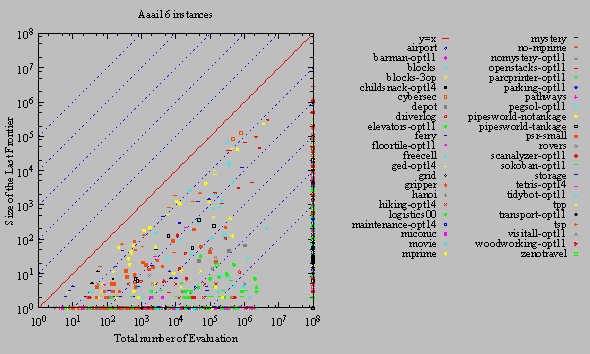
\includegraphics{tables/aaai16-front-vs-evaluated.pdf}
 \caption{Comparison of the size of the search plateau compared to the total evaluation. Data were obtained by the result of standard FIFO tiebreaking on the standard benchmark instances. Both axes are logarithmic. Each dotted line represents 10x, 100x ... lines.  Openstacks,  clearly has the large plateaus.}
 \label{plateau-h}
\end{figure}
% 
% \begin{figure}[htbp]
%  \centering
%  \relsize{-2}
%  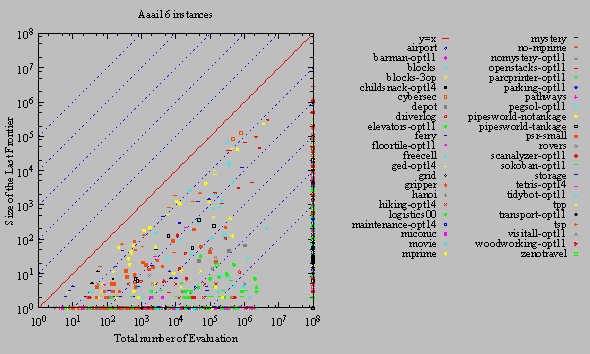
\includegraphics{tables/aaai16-front-vs-evaluated.pdf}
%  \caption{Comparison of the size of the search plateau compared to the total evaluation. Data were obtained by the result of running \astar on the standard benchmark instances, with FIFO but without the tiebreaking by $h$. Both axes are logarithmic. Each dotted line represents 10x, 100x ... lines.}
%  \label{plateau-f}
% \end{figure}


We can have several important observations from these results.  Firstly, in a plateau, \textbf{the heuristic functions are not used at all, nor the search is guided at all}. This observation holds even if we combine several nondominating heuristics for tie breaking e.g. \lmcut and M\&S.  It is still possible that a plateau is encountered, since their combination is not a perfect heuristics yet!

Secondly, such a plateau is known to be inevitable even if we have an almost perfect heuristics $h_c$, and it is impossible to improve upon $h_c$ --- if it could, the result would be a perfect heuristics or an inadmissible heuristics. Therefore, this problem \textbf{cannot be solved by improving the heuristic accuracy, which is the currently dominating meta-strategy to improve the planner performance.}  Note that combining multiple heuristic functions by taking their maximum is still an attempt to improve the accuracy, therefore it does not solve this problem.

Thirdly, there is no legitimate reason which supports each tiebreaking strategy. \textbf{$h$ and FIFO are just heuristically chosen by the implementer of the planner.} Nor are there any reason to choose LIFO, or Random tie breaking. Moreover, the different seed value of a Random tiebreaking yield the different search behavior and different result. (In all of our experiment we fixed the seed to 1.)

% Based on these observation, the next step we have taken is to develop a new
% portfolio-based multi-tiebreaking strategy \textbf{which is orthogonal to
% the approach of improving the heuristic accuracy.}

\section{Domains with Large Plateau}

Currently, most benchmark domains except Openstacks and Cybersec do not
have the large plateau thanks to the powerful heuristic
estimates. However, limiting our effective experiments only to 2 domains
would bias our observation. To avoid this issue, we created several
domains where the \sota heuristic functions fail to provide a
menaingful guidance.

One important characteristics shared by Openstacks and Cybersec is that they both
have large number of zero-cost actions. In such situations, both LMcut
and M\&S fail to find a meaningful heuristic estimate because LMcut fails to
find a good cost partitioning with non-zero values, and most edges in the abstraction space of
M\&S have zero costs.

We therefore modified various domains to have many zero-cost actions.
For example, miconic-up is a domain which minimizes the energy
consumption caused by ``up'' action, which moves the elevator up, and
all other actions have zero-cost. Another example is driverlog-fuel, where only
the ``drive'' action has cost 1 and all other actions are zero-cost.
This in fact reflects the practical application compared to the original
unit-cost domains where driving and manual labor is equally accounted.
Oddly, although some planners have options which treats actions as if
they are unit-costs, and describe such options as ``inadmissible'',
solving domains which are unit-cost by origin is not called
``inadmissible''. Above domain modification addresses this problem.

Modification was mainly conducted so that it is practically reasonable
in a sense of cost minimization. Most transportation-type domains are
modified so that they use less fuel. Assembly-type domains are modified
so that it minimizes the resource usage such as ink or wood.

\section{Depth-based Tiebreaking}

In order to solve this kind of problem with the large final plateau, the
planner needs to run an efficient knowledge-free search within plateau.
One useful measure for such situation might be the number of steps from
the entrance of the plateau.

The \emph{depth} of a node is an integer equal to the depth of its
parent node plus one. If the parent node is from the other plateau,
e.g., different $f$-value, or different $h$-value used for the first
tiebreaking, the depth is 0. Nodes are stored in a bucket each associated with
particular depth.

This method is very similar to inadmissible search technique in LAMA
planner \cite{richter2010lama} which increases every action costs by 1,
called PLUSONE cost-type.
It is explicitly targeted at zero-cost actions observed in Openstacks, and resulted in a
significantly better performance in IPC-6.

The major difference of our tiebreaking from there strategy is twofold. First, the
depth used for tiebreaking does not affect the cost, thus does not lose
the admissibility. Next, we \emph{do not favor smaller depth over
higher depth} --- In PLUSONE, three successive applications of zero-cost operators result in
cost 3, and two applications result in a cost 2, and smaller cost is
preferred, just as \astar always expands the node with smaller $f$-value.
However, in the knowledge-free search within the plateau of admissible search,
all nodes have the same $f$-value
and it is impossible to guess whether the goal is near the entrance or
far away from the entrance.
In the formar case, the search should be focused around the entrance
(smaller depths). However, in the latter case, the planner should
greedily explore the various area of the plateau by preferring larger depth.
This ``greediness'' is different from the normal sense of ``greedy
search'' --- since this greediness only holds within the plateau,
admissibility is still maintained.



\section{Related Work}
\label{sec-4}

\emph{Symmetry Breaking} \cite{Fox1998,pochter2011exploiting,domshlak2013symmetry} is the search technique that tries to prune the states with symmetric paths. \emph{Partial Order Reduction}, \emph{Strong Stubbern Sets} and \emph{Expansion Core} are also the techniques which prune the intermediate states that reach to the same goal using the different orders of same actions. \emph{Dominance Pruning} \cite{erol1994} is a technique which exploits additional information from the problem after the heuristics are computed. Instead of computing the absolute distance, it  proves if a state is strictly relatively better than the other nodes.

LA* is an extension of \astar which employs a \emph{lookahead} to each
expansion of a node. Lookahead is a Depth First Search from the frontier
node which allows to find nodes whose 

\section{Conclusion}

In this paper, we proposed two novel diversity-aware tie-braking methods for the admissible search using \astar. We empirically showed that they improve the performance on various domains, and they are heuristic-agnostic improvements. We showed that they have a significant impact on the final step of the search in large plateau.
 % when the distribution of optimal solutions is not uniform within the open list.
% We also showed that this nonuniform distribution still appears when we have almost-perfect % heuristics.

Our method differs from the other pruning techniques such as symmetry breaking, dominance pruning or partial-order-pruning because we actually do not prune any states, nor from the other general improvements in the heuristic accuracy because we just change the expansion order within the same $f$.
